
\documentclass{book}

\usepackage{graphicx}
\usepackage{hyperref}

\title{Maps and Notes to Supplement Churchill's {\it A History of the
English-Speaking Peoples\/}}

\author{Thomas E.~Vaughan}

\begin{document}

\frontmatter

\maketitle

\chapter{Preface}

Winston Churchill's {\it A History of the English-Speaking Peoples}, at least
in its abridgment for the American audience, is an excellent history, but it
lacks maps. A reader like me will have some difficulty in visualizing the
location of one or another event because of his unfamiliarity with geography
and with the evolution of place names over time. The present work is an effort
to provide a visual reference for Churchill's book.

\mainmatter%

\chapter{Britannia}

On Page~1 is a reference to Gaul, which Julius Caesar had in 55~BC just
finished conquering. Figure~\ref{fig:gaul-bc} depicts the Roman view of Gaul at
the time. Gaul then covered the territory now covered by France, Luxembourg,
Belgium, part of the Netherlands, and part of Germany.  At this time, Caesar
turned his attention to Brittania, whose people were of the same general,
Celtic culture as those in Gaul. Churchill writes, ``The Islanders had helped
the local tribes in the late campaigns along the northern coast of Gaul\ldots.
British volunteers had shared the defeat of the Veneti on the coasts of
Brittany in the previous year.'' The location of the Veneti is indicated in
Figure~\ref{fig:gaul-bc}, and Brittany is located in Figure~\ref{fig:brittany}.

\begin{figure}
   \begin{center}
      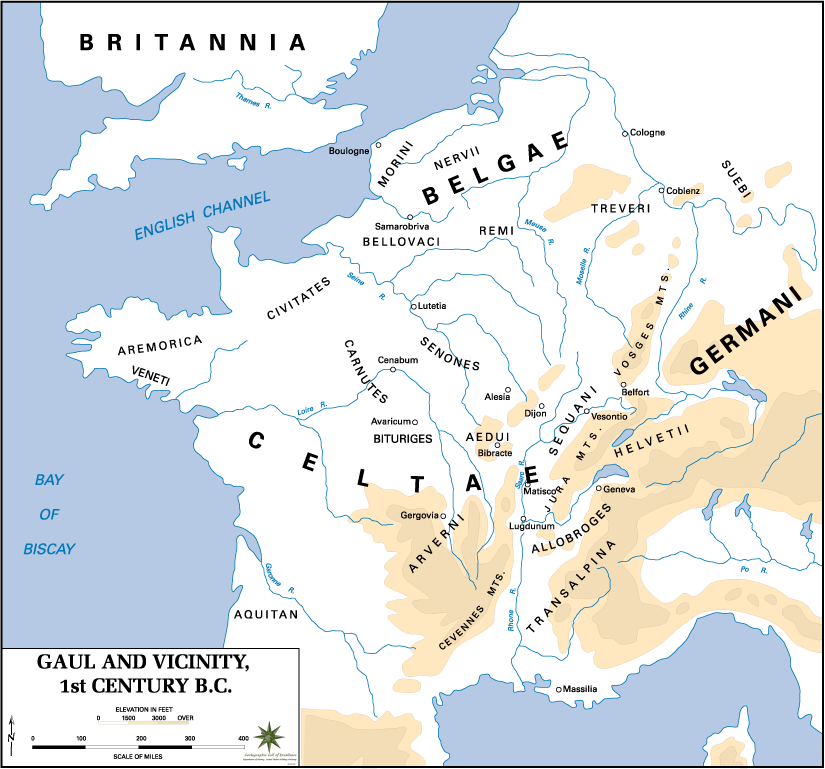
\includegraphics[width=0.9\textwidth]{images/Gaul-1st-century-BC}
      \caption{%
         Gaul as viewed by the Romans in the First Century BC\@.
         \url{http://en.wikipedia.org/wiki/Gauls}%
      }\label{fig:gaul-bc}
   \end{center}
\end{figure}

\begin{figure}
   \begin{center}
      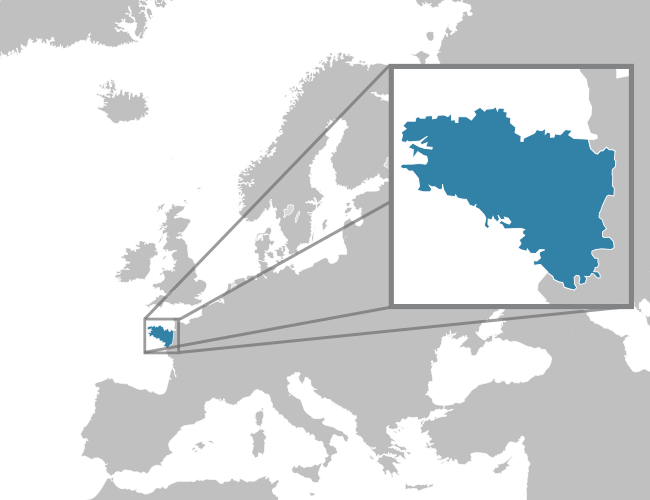
\includegraphics[width=0.9\textwidth]{Bretagne}
      \caption{%
         Brittany's location in northwest France\@.
         \url{http://en.wikipedia/org/wiki/Brittany}
      }\label{fig:brittany}
   \end{center}
\end{figure}

On Page~2 is a reference to Caesar's timber bridge across the Rhine above
Coblenz, whose location can be found in Figure~\ref{fig:gaul-bc}. A magnified
view is provided in Figure~\ref{fig:Rhine-Crossing}. The bridge is regarded as
a marvel of military engineering. After the bridge was destroyed, Caesar
marched his troops westward to the shore somewhere between Boulogne and Calais.
The location of Boulogne can be found in Figure~\ref{fig:gaul-bc}. The location of
Calais can be found in Figure~\ref{fig:LondonCalaisParis}

\begin{figure}
   \begin{center}
      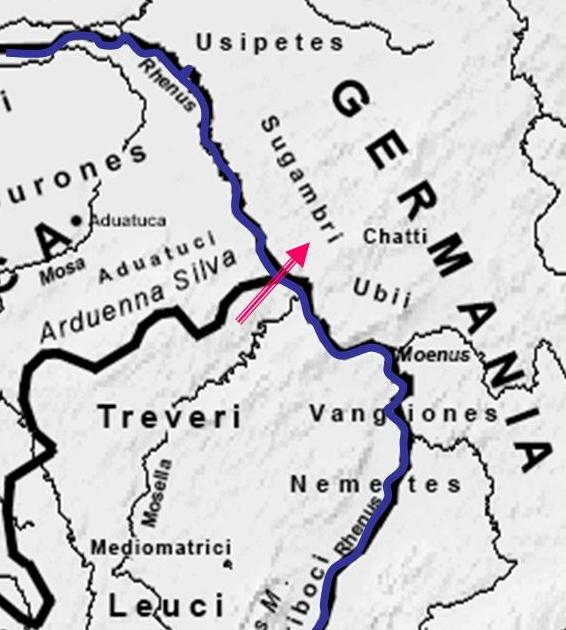
\includegraphics[width=0.9\textwidth]{images/Rhine-Crossing.jpg}
      \caption{%
         Location of Caesar's Rhine crossing\@.
         \url{http://en.wikipedia/org/wiki/Caesar's_Rhine_bridges}
      }\label{fig:Rhine-Crossing}
   \end{center}
\end{figure}

\begin{figure}
   \begin{center}
      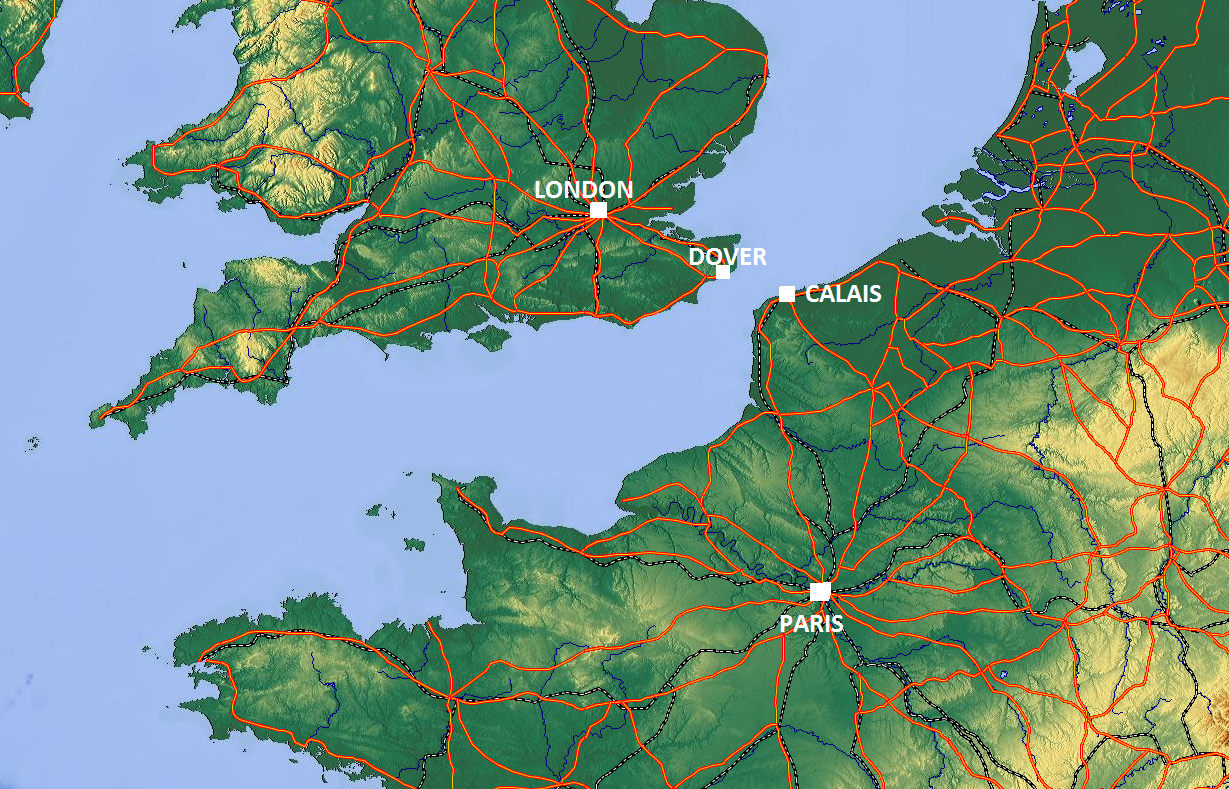
\includegraphics[width=0.9\textwidth]{images/LondonCalaisParis.png}
      \caption{%
         Location of Calais\@.
         \url{http://en.wikipedia/org/wiki/Calais}
      }\label{fig:LondonCalaisParis}
   \end{center}
\end{figure}

\backmatter%

\end{document}

